O método de Interpolação Polinomial é mais um método numérico iterativo para minimização de funções. 

\begin{figure}[h]
	\begin{center}	
		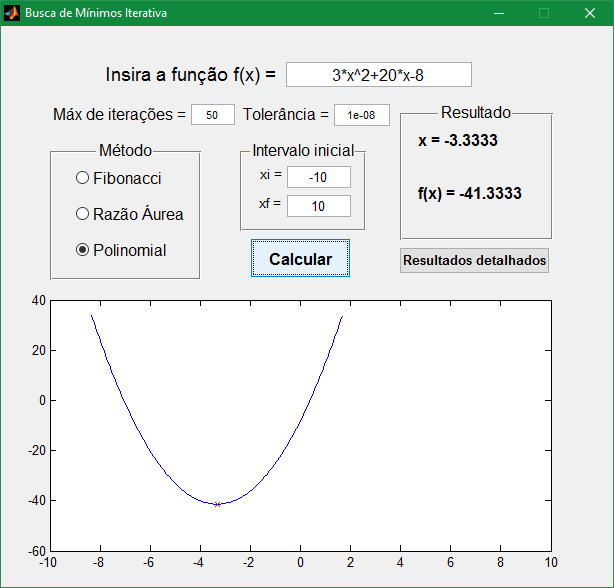
\includegraphics[width=14cm]{../interpol/f1_gui.PNG}
		\caption{escrevaaquiseucaption}
		\label{fig:f1_gui}
	\end{center}
\end{figure}

\begin{figure}[H]
	\begin{center}	
		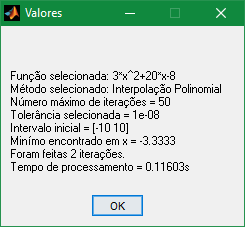
\includegraphics[width=6cm]{../interpol/f1_resultados.PNG}
		\caption{escrevaaquiseucaption}
		\label{fig:f1_resultados}
	\end{center}
\end{figure}

\begin{figure}[H]
	\begin{center}	
		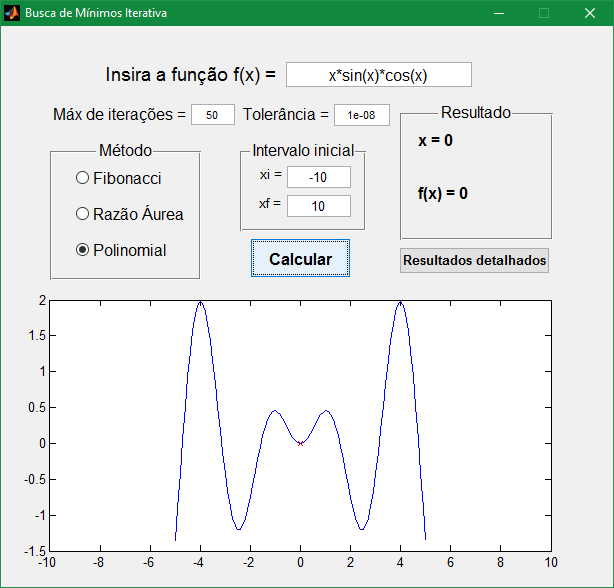
\includegraphics[width=14cm]{../interpol/f2_gui.PNG}
		\caption{escrevaaquiseucaption}
		\label{fig:f2_gui}
	\end{center}
\end{figure}

\begin{figure}[H]
	\begin{center}	
		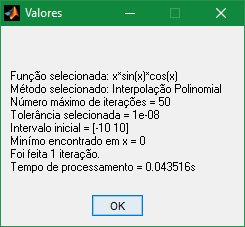
\includegraphics[width=6cm]{../interpol/f2_resultados.PNG}
		\caption{escrevaaquiseucaption}
		\label{fig:f2_resultados}
	\end{center}
\end{figure}

\begin{figure}[H]
	\begin{center}	
		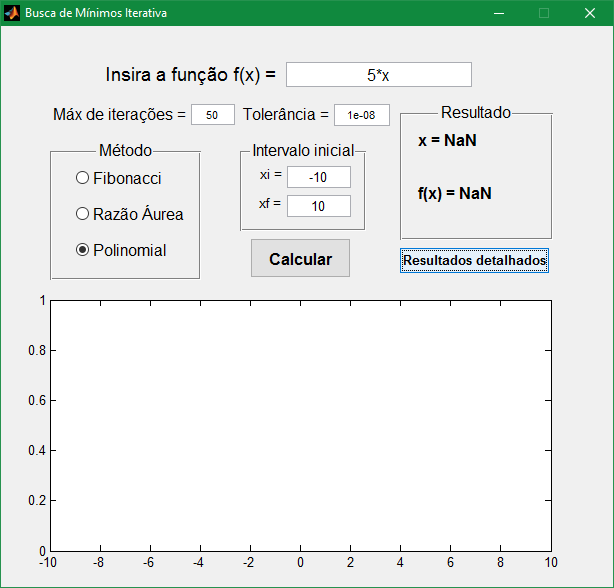
\includegraphics[width=14cm]{../interpol/f3_gui.PNG}
		\caption{escrevaaquiseucaption}
		\label{fig:f3_gui}
	\end{center}
\end{figure}

\begin{figure}[H]
	\begin{center}	
		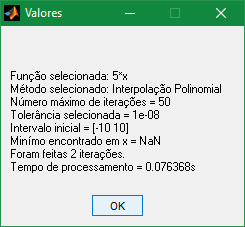
\includegraphics[width=6cm]{../interpol/f3_resultados.PNG}
		\caption{escrevaaquiseucaption}
		\label{fig:f3_resultados}
	\end{center}
\end{figure}

\begin{figure}[H]
	\begin{center}	
		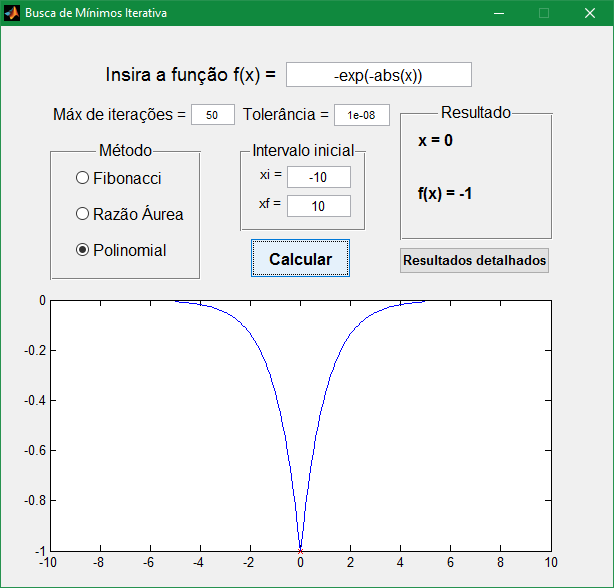
\includegraphics[width=14cm]{../interpol/f4_1_gui.PNG}
		\caption{escrevaaquiseucaption}
		\label{fig:f4_1_gui}
	\end{center}
\end{figure}

\begin{figure}[H]
	\begin{center}	
		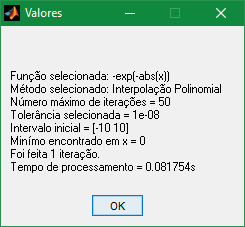
\includegraphics[width=6cm]{../interpol/f4_1_resultados.PNG}
		\caption{escrevaaquiseucaption}
		\label{fig:f4_1_resultados}
	\end{center}
\end{figure}

\begin{figure}[H]
	\begin{center}	
		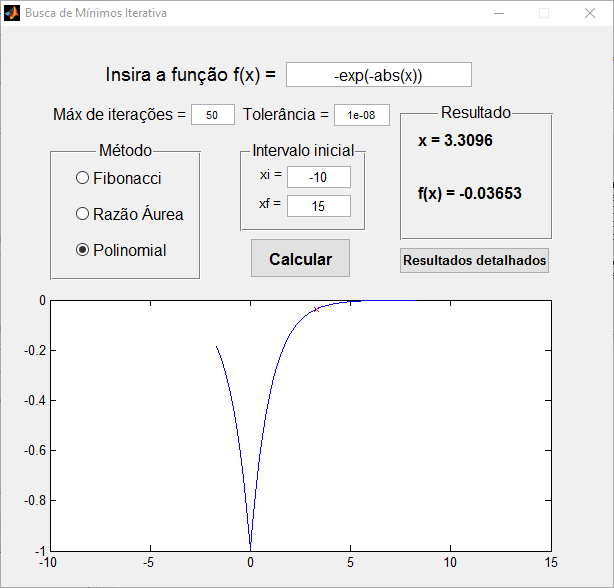
\includegraphics[width=14cm]{../interpol/f4_2_gui.PNG}
		\caption{escrevaaquiseucaption}
		\label{fig:f4_2_gui}
	\end{center}
\end{figure}

\begin{figure}[H]
	\begin{center}	
		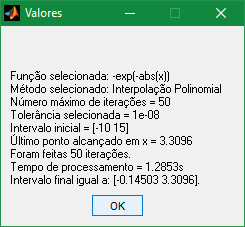
\includegraphics[width=6cm]{../interpol/f4_2_resultados.PNG}
		\caption{escrevaaquiseucaption}
		\label{fig:f4_2_resultados}
	\end{center}
\end{figure}

